Các bối cảnh giới hạn phải độc lập trong bối cảnh riêng và có mô hình miền riêng, nhưng các bối cảnh giới hạn cần tương tác, giao tiếp để trao đổi thông tin. Vì vậy các bối cảnh giới hạn có thể có mối quan hệ với nhau. Những mối quan hệ này cần được quản lý chặt chẽ để hoạt động độc lập, nhất quán và linh hoạt. Do đó, cần phải ghi lại các mối quan hệ thông qua việc sử dụng bản đồ bối cảnh. \emph{Bản đồ bối cảnh (Context Maps)} là sự thể hiện trực quan của hệ thống, thể hiện các thành phần và mối quan hệ giữa các thành phần.


\begin{figure}[H]

    \centering
    
    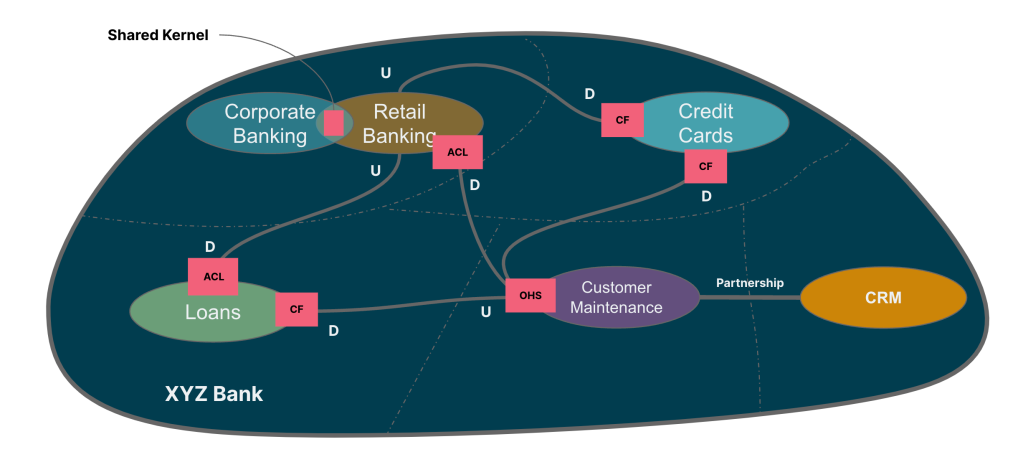
\includegraphics[scale = 0.5]{pictures/ban_do_boi_canh/main.drawio.png}
    
    \caption{vvn20206205}
    
    \end{figure}